\documentclass[tikz]{standalone}

\usetikzlibrary{calc}
\usetikzlibrary{shapes}

\definecolor{c1}{RGB}{62,91,90}
\definecolor{c2}{RGB}{103,152,149}
\definecolor{c3}{RGB}{194,214,213}
\definecolor{c4}{RGB}{0,255,255}

\begin{document}
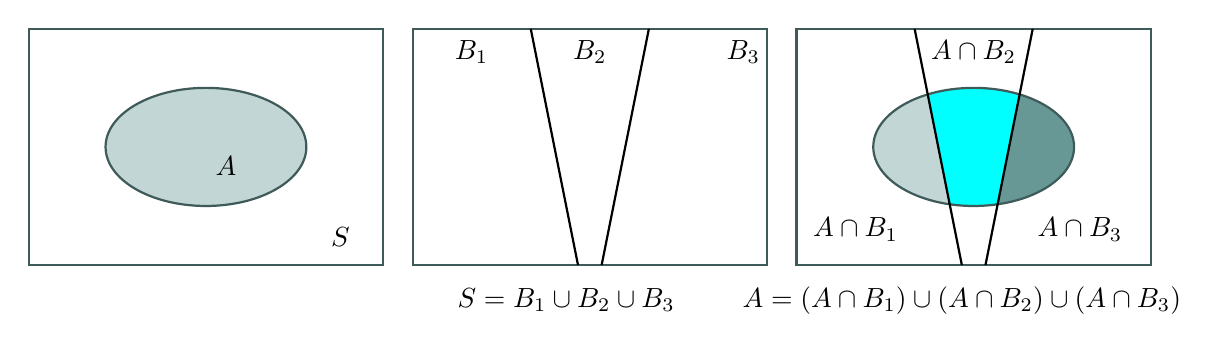
\begin{tikzpicture}[scale=1.5]
    \begin{scope} %1st pic
        \draw[draw=c1,thick] (0,0) rectangle (3,2);
        \draw[draw=c1,thick,fill=c3] (1.5,1) ellipse (0.85 and 0.5);
        \node[below right] at (1.5,1) {$A$};
        \node[below left] at (2.8,0.4) {$S$};
    \end{scope}
    % second picture, shift to the right 3.5 cm, bigger than the bounding rectangle (3,2)
    \begin{scope}[xshift=3.25cm] %intersection
        \coordinate (A1) at (1.4,0);
        \coordinate (A2) at (1.6,0);
        \coordinate (B1) at (1,2);
        \coordinate (B2) at (2,2);
        \draw[draw=c1,thick] (0,0) rectangle (3,2);
        \draw[thick] (A1) -- (B1);
        \draw[thick] (A2) -- (B2);
        \node[] at (0.5,1.8) {$B_1$};
        \node[] at (1.5,1.8) {$B_2$};
        \node[] at (2.8,1.8) {$B_3$};
        \node[] at (1.3,-0.3) {$S=B_1 \cup B_2 \cup B_3$};
    \end{scope}
    % third pic
   \begin{scope}[xshift=6.5cm] %intersection
     \coordinate (A1) at (1.4,0);
        \coordinate (A2) at (1.6,0);
        \coordinate (B1) at (1,2);
        \coordinate (B2) at (2,2);
        \draw[draw=c1,thick] (0,0) rectangle (3,2);
   
        \begin{scope}
            \clip (0,0)--(A1)--(B1)--(0,2)--cycle;
            \draw[draw=c1,thick,fill=c3] (1.5,1) ellipse (0.85 and 0.5);
        \end{scope}
        \begin{scope}
            %\clip (0,0)--(A1)--(B1)--(0,2)--cycle;
            \clip (A1)--(A2)--(B2)--(B1);
            \draw[draw=c1,thick,fill=c4] (1.5,1) ellipse (0.85 and 0.5);
        \end{scope}
        \begin{scope}
            %\clip (0,0)--(A1)--(B1)--(0,2)--cycle;
            \clip (A2)--(3,0)--(3,2)--(B2);
            \draw[draw=c1,thick,fill=c2] (1.5,1) ellipse (0.85 and 0.5);
        \end{scope}
        \draw[thick] (1.4,0) -- (1,2);
        \draw[thick] (1.6,0) -- (2,2);
        \node[] at (.5,0.3) {$A \cap B_1$};
        \node[] at (2.4,0.3) {$A \cap B_3$};
        \node[] at (1.5,1.8) {$A \cap B_2$};
        \node[] at (1.4,-0.3) {$A = (A \cap B_1) \cup ( A \cap B_2) \cup (A\cap B_3) $};
    \end{scope}
 
\end{tikzpicture}
\end{document}

